\newcommand{\run}[1]{#1-aviI}
\newcommand{\RUN}{\aviI:\;}


%%....................................F.I.G.U.R.E.............................................
\begin{figure}
\includegraphics[]{tracks-age-aviI_shrunk2prepress}
\caption{\MI: Cyclones in red. Tracks younger than $1a$ omitted for clarity.}
\label{fig:tracks-age-aviI_shrunk2prepress}
\end{figure}
%%....................................F.I.G.U.R.E.............................................

\newthought{The results } from the \MI -method are special in that they feature many long-lived eddies (see \cref{fig:histTrackCount-aviI,fig:tracks-age-aviI_shrunk2prepress,fig:defl-age-aviI_shrunk2prepress}),
some of which traveled more than $4000$ km west.
Tracks were recorded throughout the entire world ocean with the only exceptions being an approximately $\deg{20}$-wide stripe along the equator. The highest count of unique eddies is along the Antarctic Circumpolar Current \footnote{abbreviated ACC from here on.} with counts of more than $60$ individual eddy-visits per $\deg{1} \times \deg{1}$-cell. Further eddy-rich regions are the western North-Atlantic throughout the Gulf-Stream and North-Atlantic Current, \textit{Mozambique eddies} \citep{Schouten2003} at $\deg{20}$ South along the Mozambique coast, along the Agulhas Current and south of the Cup of Good Hope at $\sim \deg{40}$, along the coasts of Brazil, Chile and all along the Eastern, Southern and Western coasts of Australia (see \cref{fig:MapVisitsBoth-aviI}).
Eddies appear and disappear throughout the world ocean. For long-lived solid eddies there is a tendency to emerge along western coasts (see \cref{fig:birthsdeathsOneYearAndMore-aviI}).

\newthought{The scale}~$\scale$ of tracked eddies is similar to that in \citet{Chelton2011}, yet generally smaller in high latitudes and slightly larger in low latitudes (see \cref{fig:ScheltsAll}). It is larger than the first-mode baroclinic Rossby Radius by a factor of at least $2$ and its meridional profile appears to be separable into two different regimes; one apparently linear profile in low latitudes and a steeper one equator-wards of $\sim \left| \deg{15} \right|$. Regionally, locations of high mesoscale activity appear to correlate with smaller eddy-scales (see \cref{fig:MapSigma-aviI}).

%%....................................F.I.G.U.R.E.............................................
\begin{marginfigure}
		\includegraphics[]{\run{histTrackCount}}
\caption[\RUN tracks.]{\RUN Final age distribution. x-axis: [days], Left y-axis: [1000]}
\label{\run{fig:histTrackCount}}
\end{marginfigure}
%%....................................F.I.G.U.R.E.............................................

\newthought{The eastward zonal drift speeds } are slightly slower than the first-mode baroclinic Rossby-Wave phase-speed and agree well with the results from \citet{Chelton2011}. Propagation is generally west-wards except for regions of sufficiently strong eastward advection as in the ACC and North Atlantic Current (see \cref{fig:velZon-aviI,fig:ScheltsAll}).


%%....................................F.I.G.U.R.E.............................................
\begin{figure}
	\includegraphics[]{\run{birthsdeathsOneYearAndMore}}
	\caption{\RUN Births are in blue and deaths in green. Size of dots scales to age squared. Only showing tracks older than one year.}
	\label{\run{fig:birthsdeathsOneYearAndMore}}
\end{figure}

%%\begin{wrapfigure}{r}{0.6\textwidth}
%\begin{marginfigure}
		%\includegraphics[width=1\linewidth]{\run{MapVisitsBoth}}
		%\caption{\RUN Total count of individual eddies per 1 degree square.}
		%\label{\run{fig:MapVisitsBoth}}
%\end{marginfigure}
%%\end{wrapfigure}
%%%....................................F.I.G.U.R.E.............................................
%\begin{marginfigure}
		%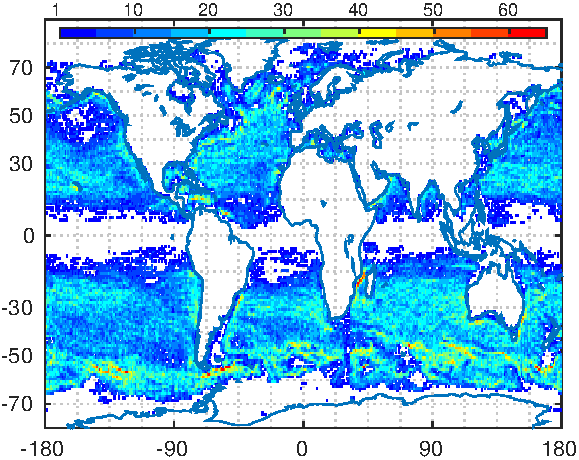
\includegraphics[width=1\linewidth]{MapVisitsBoth-aviII}
		%\caption{\aviII: Total count of individual eddies per 1 degree square.}
		%\label{fig:MapVisitsBoth-aviII}
%\end{marginfigure}
%%%....................................F.I.G.U.R.E.............................................
%\begin{figure*}
		%\includegraphics[]{\run{MapSigma}}
		%\caption{\RUN \capS}
	%\label{\run{fig:MapSigma}}
%\end{figure*}
%%....................................F.I.G.U.R.E.............................................

%%....................................F.I.G.U.R.E.............................................
%\begin{figure*}
		%\includegraphics[]{\run{velZon}}
		%\caption{\RUN \capU }
	%\label{\run{fig:velZon}}
%\end{figure*}
%%....................................F.I.G.U.R.E.............................................
